% =========================================================================
% HOW TO USE THIS TEMPLATE
%
% A reference chapter, not part of a thesis. Delete the \include line in
% main.tex and this folder once you no longer need it.
%
% Derivation notice (LPPL clause 6b): the table examples in this file
% (the tabular and tabularx subsections, their captions and sample rows)
% are adapted from the LaTeX tutorial chapter of the "IPLeiria Thesis"
% template v2.1.0 by Jose Antonio Portela Areia (LPPL-1.3c). Everything
% else was written for this template, and the adapted examples were
% reworded and restyled for ICS-ULisboa. See NOTICE.
% =========================================================================

\chapter{How to Use This Template}
\label{ch:how-to}

Everything shown here compiles in this document, so if an example looks
right on the page it will look right in your thesis.

\section{Tables}
\label{sec:tables}

Captions go above tables, as rule 4.5 requires. Each table must sit inside
a \verb|\begin{table}| environment; the \verb|[!htpb]| float options give
the best placement, and the same advice applies to figures.

\subsection{Tabular Environment}

The conventional \verb|\begin{tabular}| environment produces a simple
table. \Cref{tab:table-01} uses \texttt{booktabs} rules, which is the
convention in the discipline. Vertical lines are not used.

\begin{table}[!htpb]
  \caption{A table showcasing the usage of the tabular environment.}
  \label{tab:table-01}
  \centering
  \begin{tabular}{llc}
    \toprule
    \textbf{Header 01} & \textbf{Header 02} & \textbf{Header 03} \\
    \midrule
    Lorem Ipsum       & Pharetra Dolor    & $\checkmark$ \\
    Amet Consectetuer & Curabitur Aliquet & --           \\
    Praesent Mauris   & Praesent Libero   & $\checkmark$ \\
    \bottomrule
  \end{tabular}
\end{table}

\subsection{Tabularx Environment}

Use \verb|\begin{tabularx}{\textwidth}{lX}| for a table with a column that
expands to fill the remaining width. \Cref{tab:table-02} shows it.

\begin{table}[!htpb]
  \caption{A table showcasing the usage of the tabularx environment.}
  \label{tab:table-02}
  \begin{tabularx}{\textwidth}{lX}
    \toprule
    \textbf{Header 01} & \textbf{Header 02} \\
    \midrule
    Lorem Ipsum   & \blindtext[1] \\
    Dolor Sit     & Quisque cursus, metus vitae pharetra auctor, sem massa
                    mattis sem, at interdum magna augue eget diam. \\
    \bottomrule
  \end{tabularx}
\end{table}

\subsection{Notes Below a Table}

The \verb|threeparttable| environment attaches notes that inherit the
width of the table, as in \Cref{tab:table-03}.

\begin{table}[!htpb]
  \caption{A table with notes attached below it.}
  \label{tab:table-03}
  \centering
  \begin{threeparttable}
    \begin{tabular}{l
                    S[table-format=1.2]
                    S[table-format=1.2]
                    S[table-format=1.2]
                    S[table-format=2.2]}
      \toprule
      \textbf{Header 01} & {\textbf{Mean}} & {\textbf{SD}} & {\textbf{Min}}
        & {\textbf{Max}} \\
      \midrule
      Lorem Ipsum       & 1.82 & 1.44 & 0.00 & 8.00 \\
      Amet Consectetuer & 0.47 & 0.29 & 0.00 & 1.00 \\
      Praesent Mauris   & 7.31 & 6.90 & 0.00 & 41.00 \\
      \bottomrule
    \end{tabular}
    \begin{tablenotes}[flushleft]
      \footnotesize
      \item \textit{Note}: Notes go here, at the width of the table.
      \item \textit{Source}: [Source of the data].
    \end{tablenotes}
  \end{threeparttable}
\end{table}

\subsection{Regression Tables}

Regression output combines several of the tools above. The \texttt{S}
columns of \texttt{siunitx} align the estimates on the decimal marker
(which becomes a comma in a thesis written in Portuguese), standard
errors in parentheses and significance stars included;
\verb|\multicolumn| and \verb|\cmidrule| group the models under a common
heading; and \texttt{threeparttable} holds the notes, as in
\cref{tab:regression}.

\begin{table}[!htpb]
  \caption{A regression table with grouped columns and notes.}
  \label{tab:regression}
  \centering
  \begin{threeparttable}
    \begin{tabular}{l
                    S[table-format=-1.3{***}, table-space-text-pre=(]
                    S[table-format=-1.3{***}, table-space-text-pre=(]
                    S[table-format=-1.3{***}, table-space-text-pre=(]}
      \toprule
      & \multicolumn{2}{c}{\textbf{Header 01}}
      & \multicolumn{1}{c}{\textbf{Header 02}} \\
      \cmidrule(lr){2-3}\cmidrule(lr){4-4}
      & {(1)} & {(2)} & {(3)} \\
      \midrule
      Lorem Ipsum       & -0.213***  & -0.198***  & -0.176**  \\
                        & (0.036)    & (0.041)    & (0.070)   \\
      Dolor Sit         &  0.048**   &  0.051**   &  0.032    \\
                        & (0.019)    & (0.020)    & (0.027)   \\
      Amet Consectetuer &            &  0.137**   &  0.140*   \\
                        &            & (0.058)    & (0.076)   \\
      \midrule
      Fixed effects     & {Yes}      & {Yes}      & {No}      \\
      Observations      & {\num{2431}}     & {\num{2398}}     & {\num{1207}}    \\
      \bottomrule
    \end{tabular}
    \begin{tablenotes}[flushleft]
      \footnotesize
      \raggedright
      \item \textit{Note}: Standard errors in parentheses.
        * $p<\num{0.10}$; ** $p<\num{0.05}$; *** $p<\num{0.01}$.
    \end{tablenotes}
  \end{threeparttable}
\end{table}

\subsection{Tables Produced in R or Stata}

Export the estimation output to a \texttt{.tex} file and pull it in with
\verb|\input{}|, keeping the caption and the label in the main document:

\begin{verbatim}
\begin{table}[!htpb]
  \caption{Caption goes here.}
  \label{tab:from-r}
  \input{Figures/table-01.tex}
\end{table}
\end{verbatim}



\subsection{Long Tables}

A table that runs over several pages, such as a list of cases or a
codebook, uses \verb|longtable| instead of \verb|table|. It cannot float,
so it starts exactly where it appears in the text; the header is repeated
at the top of every page, as \cref{tab:longtable} shows. Wide tables are
rotated rather than shrunk: see \cref{sec:landscape}.

\begin{longtable}{lS[table-format=1.2]S[table-format=1.2]S[table-format=2.0]}
  % No space or line break between \caption, \label and \\: in a long
  % table a stray space shifts the caption sideways.
  \caption{A table that runs over more than one page.}\label{tab:longtable}\\
  \toprule
  \textbf{Header 01} & {\textbf{Mean}} & {\textbf{SD}} & {\textbf{N}} \\
  \midrule
  \endfirsthead
  \multicolumn{4}{l}{\textit{\tablename~\thetable\ (continued)}} \\
  \toprule
  \textbf{Header 01} & {\textbf{Mean}} & {\textbf{SD}} & {\textbf{N}} \\
  \midrule
  \endhead
  \midrule
  \multicolumn{4}{r}{\textit{(continued on the next page)}} \\
  \endfoot
  \bottomrule
  \endlastfoot
    Row 01 & 0.48 & 0.29 & 32 \\
    Row 02 & 2.37 & 1.91 & 10 \\
    Row 03 & 0.11 & 0.07 & 30 \\
    Row 04 & 3.45 & 2.79 & 19 \\
    Row 05 & 1.17 & 0.86 & 17 \\
    Row 06 & 0.53 & 0.32 & 37 \\
    Row 07 & 2.42 & 1.93 & 15 \\
    Row 08 & 0.16 & 0.09 & 35 \\
    Row 09 & 3.50 & 2.81 & 24 \\
    Row 10 & 1.22 & 0.89 & 22 \\
    Row 11 & 0.58 & 0.34 & 42 \\
    Row 12 & 2.47 & 1.96 & 20 \\
    Row 13 & 0.21 & 0.12 & 40 \\
    Row 14 & 3.55 & 2.84 & 29 \\
    Row 15 & 1.27 & 0.91 & 27 \\
    Row 16 & 0.63 & 0.37 & 47 \\
    Row 17 & 2.52 & 1.98 & 25 \\
    Row 18 & 0.26 & 0.14 & 45 \\
    Row 19 & 3.60 & 2.87 & 34 \\
    Row 20 & 1.32 & 0.94 & 32 \\
    Row 21 & 0.68 & 0.39 & 52 \\
    Row 22 & 2.57 & 2.01 & 30 \\
    Row 23 & 0.31 & 0.17 & 50 \\
    Row 24 & 3.65 & 2.89 & 39 \\
    Row 25 & 1.37 & 0.96 & 37 \\
    Row 26 & 0.73 & 0.42 & 57 \\
    Row 27 & 2.62 & 2.04 & 35 \\
    Row 28 & 0.36 & 0.19 & 55 \\
    Row 29 & 3.70 & 2.92 & 44 \\
    Row 30 & 1.42 & 0.99 & 42 \\
    Row 31 & 0.78 & 0.44 & 62 \\
    Row 32 & 2.67 & 2.06 & 40 \\
    Row 33 & 0.41 & 0.22 & 60 \\
    Row 34 & 3.75 & 2.94 & 49 \\
    Row 35 & 1.47 & 1.01 & 47 \\
    Row 36 & 0.83 & 0.47 & 67 \\
    Row 37 & 2.72 & 2.08 & 45 \\
    Row 38 & 0.46 & 0.24 & 65 \\
    Row 39 & 3.80 & 2.96 & 54 \\
    Row 40 & 1.52 & 1.04 & 52 \\
    Row 41 & 0.88 & 0.49 & 72 \\
    Row 42 & 2.77 & 2.11 & 50 \\
    Row 43 & 0.51 & 0.27 & 70 \\
    Row 44 & 3.85 & 2.99 & 59 \\
    Row 45 & 1.57 & 1.06 & 57 \\
\end{longtable}

\section{Figures}
\label{sec:figures}

Captions go below figures and are centred, as rule 4.6 requires. Give the
width relative to \verb|\linewidth| rather than in centimetres, so that
the figure rescales if the geometry changes. When a caption is too long for
the list of figures, give a short version in the optional argument of
\verb|\caption|.

\begin{figure}[!htpb]
  \centering
  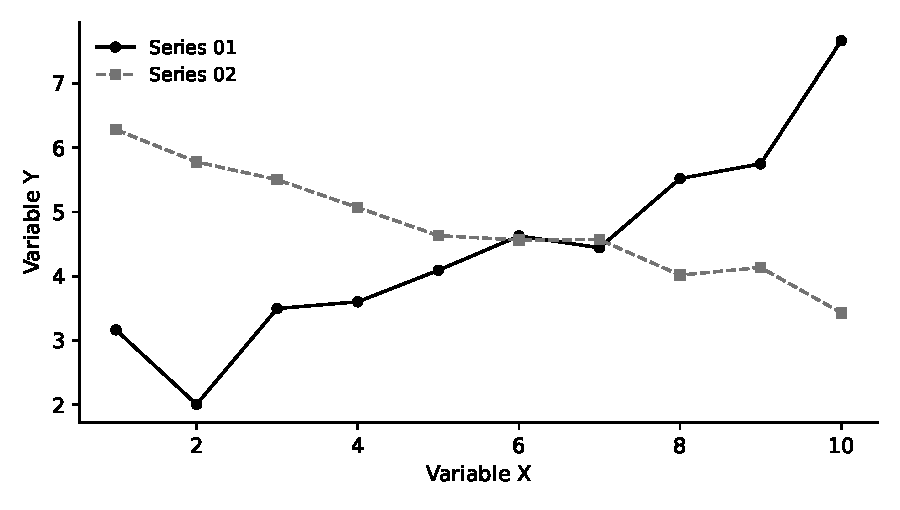
\includegraphics[width=0.85\linewidth]{Figures/example-figure.pdf}
  \caption{A figure included from a PDF file.}
  \label{fig:figure-01}
  \par\vspace{2pt}
  {\footnotesize\textit{Source}: [Source of the data].\par}
\end{figure}

As in \cref{fig:figure-01}, a note or the source of a figure goes in a
short line below the caption.

Side-by-side figures use \verb|\begin{subfigure}| inside a
\verb|\begin{figure}|. The panels can be referenced individually, as
\Cref{fig:figure-02.1} and \Cref{fig:figure-02.2}.

\begin{figure}[!htpb]
  \centering
  \begin{subfigure}{0.45\textwidth}
    \centering
    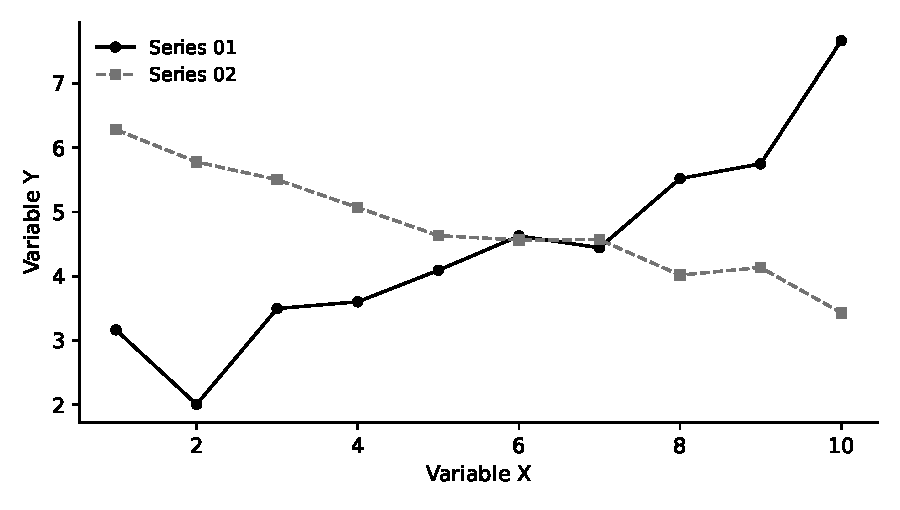
\includegraphics[width=\textwidth]{Figures/example-figure.pdf}
    \caption{Caption for figure 1.}
    \label{fig:figure-02.1}
  \end{subfigure}
  \hfill
  \begin{subfigure}{0.45\textwidth}
    \centering
    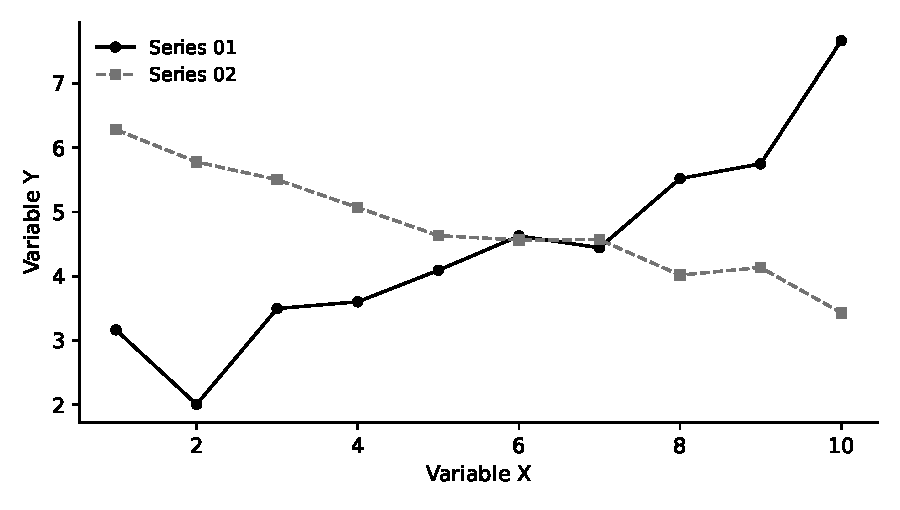
\includegraphics[width=\textwidth]{Figures/example-figure.pdf}
    \caption{Caption for figure 2.}
    \label{fig:figure-02.2}
  \end{subfigure}
  \caption{Overall caption of the figure.}
  \label{fig:figure-02}
\end{figure}

Export figures from R as PDF rather than PNG whenever they are made of
lines and text: the difference is visible in print.

\subsection{Figures Drawn in \LaTeX}

Figures can also be drawn directly with \texttt{pgfplots}, which is
loaded, so that the fonts match the body text exactly and the figure
needs no external file. \Cref{fig:coefplot} is a coefficient plot, the
graphical counterpart of \cref{tab:regression}.

\begin{figure}[!htpb]
  \centering
  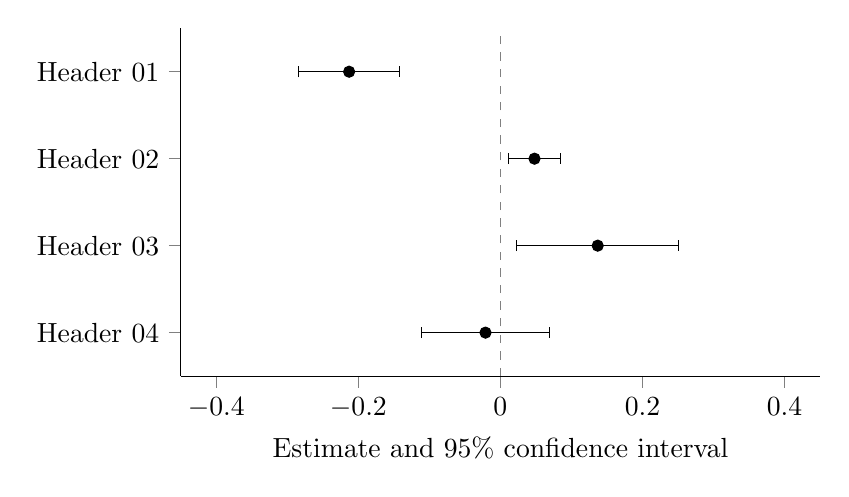
\begin{tikzpicture}
    \begin{axis}[
        width=0.8\linewidth, height=6cm,
        xmin=-0.45, xmax=0.45,
        ymin=0.5, ymax=4.5,
        ytick={1,2,3,4},
        yticklabels={Header 04, Header 03, Header 02, Header 01},
        xlabel={Estimate and 95\% confidence interval},
        axis x line*=bottom, axis y line*=left,
        tick align=outside]
      \draw[gray, dashed] (axis cs:0,0.5) -- (axis cs:0,4.5);
      \addplot[only marks, mark=*, black, mark options={fill=black},
                error bars/.cd, x dir=both, x explicit]
        coordinates {
          (-0.213,4) +- (0.071,0)
          ( 0.048,3) +- (0.037,0)
          ( 0.137,2) +- (0.114,0)
          (-0.021,1) +- (0.090,0)
        };
    \end{axis}
  \end{tikzpicture}
  \caption{A coefficient plot drawn with \texttt{pgfplots}.}
  \label{fig:coefplot}
\end{figure}

\section{Hypotheses}
\label{sec:hypotheses}

The \verb|hypotheses| list, defined by the class, numbers hypotheses as
H1, H2, and so on. Label each item and refer to it with \verb|\cref|,
which supplies the word: \cref{hyp:one} and \cref{hyp:two}.

\begin{hypotheses}
  \item \label{hyp:one} [Statement of the first hypothesis.]
  \item \label{hyp:two} [Statement of the second hypothesis.]
\end{hypotheses}

\section{Equations}
\label{sec:equations}

A single numbered equation is shown as \cref{eq:example} in
\cref{ch:study-one}. For a derivation over several lines, use
\verb|align|; the lines are aligned on the \verb|&| sign and each line
that carries a \verb|\label| is numbered, as in \cref{eq:align}.

\begin{align}
  \Pr(y_i = 1) &= \Lambda(\alpha + \beta x_i) \nonumber \\
               &= \frac{\exp(\alpha + \beta x_i)}
                       {1 + \exp(\alpha + \beta x_i)}.
  \label{eq:align}
\end{align}

\section{Footnotes}
\label{sec:footnotes}

Footnotes are numbered continuously through the document and set as the
regulation asks; see the example in \cref{ch:study-one}. A footnote can
carry a citation like any other text.\footnote{See \textcite{sartori1970}
and, for a different view, \textcite[690]{lijphart1971}.} Place the
footnote mark after the punctuation.

\section{Quotations and Other Languages}
\label{sec:quotations}

Two commands from \texttt{csquotes} and \texttt{babel} take care of
quotation marks and of passages in other languages:

\begin{description}[style=nextline, leftmargin=1cm, font=\normalfont\ttfamily]
  \item[\textbackslash enquote\{...\}] A short quotation, with the
    quotation marks of the language of the passage:
    \enquote{Lorem ipsum dolor sit amet}.
  \item[\textbackslash foreignlanguage\{portuguese\}\{...\}] A passage in
    another language, with the hyphenation and quotation marks of that
    language: \foreignlanguage{portuguese}{\enquote{Lorem ipsum dolor sit
    amet}}.
\end{description}

Longer quotations are set apart with the \verb|quote| environment, as in
\cref{ch:study-two}.

\section{Citations and References}
\label{sec:citations}

The bibliography is APA, produced by \texttt{biblatex} with the
\texttt{biber} backend. Chicago author-date is the other style the ICS
accepts; to switch, comment out the APA block in \texttt{icsthesis.cls}
and uncomment the Chicago block below it.

\begin{table}[!htpb]
  \caption{Citation commands.}
  \label{tab:table-04}
  \begin{tabularx}{\textwidth}{>{\ttfamily\footnotesize}l X}
    \toprule
    \textrm{\normalsize\textbf{Command}} & \textbf{Output} \\
    \midrule
    \textbackslash parencite\{key\}          & \parencite{hirschman1970} \\
    \textbackslash textcite\{key\}           & \textcite{hirschman1970} \\
    \textbackslash parencite[45]\{key\}      & \parencite[45]{hirschman1970} \\
    \textbackslash parencite[see][12]\{key\} & \parencite[see][12]{katzmair1995} \\
    \textbackslash parencite\{a,b\}          & \parencite{sartori1970,lijphart1971} \\
    \textbackslash citeyear\{key\}           & \citeyear{tsebelis2002} \\
    \textbackslash citeauthor\{key\}         & \citeauthor{tsebelis2002} \\
    \midrule
    \multicolumn{2}{l}{\textrm{\normalsize\textit{Other entry types}}} \\
    \textbackslash parencite\{thesis\}       & \parencite{placeholderthesis} \\
    \textbackslash parencite\{dataset\}      & \parencite{placeholderdataset} \\
    \textbackslash parencite\{web page\}     & \parencite{ics2026} \\
    \bottomrule
  \end{tabularx}
\end{table}

The \texttt{natbib} spellings \verb|\citep| and \verb|\citet| also work,
because \texttt{biblatex} is loaded in compatibility mode. Entry types for
theses, datasets and web pages are shown in
\path{Bibliography/references.bib}.

\section{Cross-References}
\label{sec:cross-references}

Label an element with \verb|\label{LABEL}| and refer to it with
\verb|\Cref{LABEL}|, which supplies the word as well as the number:
\Cref{ch:introduction}, \Cref{sec:tables}, \Cref{tab:table-01},
\Cref{fig:figure-01}, \Cref{eq:example} and \Cref{hyp:one}. Use \verb|\cref{}| in
lowercase for a mid-sentence reference.

\section{Lists}
\label{sec:lists}

\begin{enumerate}
  \item A numbered list, useful for hypotheses.
  \begin{enumerate}
    \item Nested levels letter themselves automatically.
  \end{enumerate}
  \item Spacing inside lists is already tightened by the class.
\end{enumerate}

\begin{itemize}
  \item A bulleted list.
  \item For items without an intrinsic order.
\end{itemize}

\begin{description}[style=nextline,leftmargin=1cm]
  \item[Header 01] \blindtext[1]
\end{description}

\section{Code}
\label{sec:code}

See \Cref{lst:code-01} in \Cref{app:b}. The \texttt{listings} package
needs no special compiler setting. It knows R and Python, among many
other languages (\verb|language=R|, \verb|language=Python|); it has no
definition for Stata, whose code is best set without the
\verb|language| option.

\section{Landscape Pages}
\label{sec:landscape}

For a table or a figure too wide for the page, wrap it in a
\verb|\begin{landscape}| environment, which rotates the whole page, both
in print and on screen. \Cref{tab:landscape} is set this way. The
environment starts a new page, so place it after the paragraph that
refers to it.

\begin{landscape}
  \begin{table}[!htpb]
    \caption{A wide table set on a landscape page.}
    \label{tab:landscape}
    \centering
    \begin{tabular}{l*{8}{S[table-format=2.1]}}
      \toprule
      & {\textbf{Header 01}} & {\textbf{Header 02}} & {\textbf{Header 03}}
      & {\textbf{Header 04}} & {\textbf{Header 05}} & {\textbf{Header 06}}
      & {\textbf{Header 07}} & {\textbf{Header 08}} \\
      \midrule
      Lorem Ipsum       & 12.4 & 18.1 &  9.7 & 22.3 & 15.0 & 11.2 & 30.5 &  8.8 \\
      Dolor Sit         & 20.9 &  7.6 & 14.3 & 10.1 & 25.4 & 19.8 &  6.2 & 17.7 \\
      Amet Consectetuer &  5.3 & 11.9 & 28.0 & 16.6 &  9.1 & 21.5 & 13.4 & 24.2 \\
      Praesent Mauris   & 16.8 & 23.2 &  7.5 & 12.9 & 18.3 &  6.4 & 27.1 & 10.6 \\
      \bottomrule
    \end{tabular}
  \end{table}
\end{landscape}

\section{What the Class Handles for You}
\label{sec:automatic}

Nothing below needs to be done by hand: 2.5 cm margins; 1.5 line spacing;
justified text; 0.7 cm paragraph indents, suppressed after headings, with
no extra space between paragraphs; page numbers in the outer bottom corner
at 1.25 cm from the edge; lowercase roman numerals before the body and
arabic numerals from the introduction onwards; every front-matter element,
chapter, the bibliography and each appendix starting on an odd page; an
unnumbered dedication; footnotes one point smaller, single spaced, with a
0.4 cm hanging indent; a single-spaced bibliography with a 0.7 cm hanging
indent; and a warning in the log if the document passes 350 pages.
